\documentclass[10pt,french]{book}
\input preambule_2013

\newcounter{exoc}
\newenvironment{exoc}{%
  \refstepcounter{exoc}\textbf{Exercice \theexoc} :\par
  \medskip}%
{\medskip}

\pagestyle{empty}

\begin{document}

\begin{center}
\begin{tabularx}{\textwidth}{|>\centering m{2.5cm}|>\centering X|>{\centering\arraybackslash} m{2.5cm}|}
	\hline
		\seconde 7 &  À rendre \textbf{au plus tard} le Mardi 5 novembre \np{2013} & \textbf{Coordonnées Fonctions} \\
	\hline
		\multicolumn{3}{|c|}{\bsc{Devoir Maison de mathématiques}} \\
	\hline
        \multicolumn{1}{|r}{\bsc{Nom}:} & \multicolumn{2}{l|}{} \\
		\multicolumn{1}{|r}{Prénom:} & \multicolumn{2}{l|}{} \\
	\hline
        \multicolumn{3}{|l|}{\bfseries Note et observations :} \\[1cm]
    \hline
\end{tabularx}
\end{center}\bigskip

\begin{exoc}
    Les points $A$ et $B$ de la figure ci-dessous ont pour coordonnées respectives $(3 \pv -1)$ et $(-1 \pv 1)$.
    \begin{enumerate}
        \item Retrouver et dessiner les axes du repère, l'origine, et les unités sur chaque axe.
        \item Placer le point $C$ de coordonnées $(2 \pv 1)$.
    \end{enumerate}
    \begin{center}
        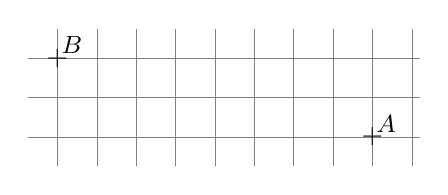
\begin{tikzpicture}[scale=0.5,>=latex]
            \draw[help lines] (-0.75,-0.75) grid (9.2,2.75);
            \draw (0,2) node {$+$} node [above right = -2pt] {\small $B$};
            \draw (8,0) node {$+$} node [above right = -2pt] {\small $A$};
        \end{tikzpicture}
    \end{center}
\end{exoc}

\begin{exoc}
    \begin{minipage}{0.6\linewidth}
    On considère le repère $(O~,~I~,~J)$ ci-contre.
        \begin{enumerate}
            \item Placer les points suivants : 
            \[A(3 \pv 1)\qq B(-2 \pv 2)\qq C(-3 \pv -1) \qetq D(4 \pv 0).\]
            \item Donner les coordonnées des points $K$ et $L$ où $K$ est le milieu de $[AB]$ et $L$ est le milieu de $[CD]$.
            \item Placer les points $K$ et $L$ sur le repère.
        \end{enumerate}
    \end{minipage}\quad
    \begin{minipage}{0.3\linewidth}
    \begin{center}
        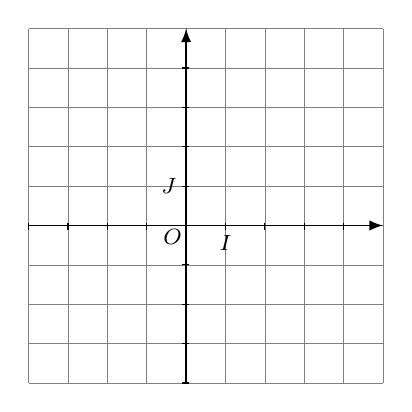
\begin{tikzpicture}[scale=0.5,>=latex]
            \draw[help lines] (-4,-4) grid (5,5);
            \coordinate (O) at (0,0); \coordinate (I) at (1,0); \coordinate (J) at (0,1);
            \draw (O) node[below left=-2pt] {\footnotesize $O$};
            \draw (I) node[below] {\footnotesize $I$};
            \draw[->,line width = 0.7pt] (-4,0) -- (5,0);
            \draw (J) node[left] {\footnotesize $J$};
            \draw[->,line width = 0.7pt] (0,-4) -- (0,5);
            \foreach \x in {-4,...,4}\draw (\x,2pt) -- (\x,-3pt);
    	\foreach \y in {-4,...,4}\draw (2pt,\y) -- (-3pt,\y);
        \end{tikzpicture}
    \end{center}
    \end{minipage}
\end{exoc}

\begin{exoc}
Que fait l'algorithme suivant? Donner une réponse précise.

\begin{center}
\small
    \psframebox{
    \parbox{0.4\linewidth}{
        \textbf{Variables}\par
            \quad $a,b,c,d,D$ : cinq nombres réels\par
        \textbf{Entrée}\par
            \quad Saisir $a$ ; Saisir $b$ ; Saisir $c$ ; Saisir $d$\par
        \textbf{Traitement}\par
            \quad Affecter à $D$ la valeur $\sqrt{(a - c)^2 + (b - d)^2}$\par
        \textbf{Sortie}\par
            \quad Afficher $D$
    }}
\end{center}
\end{exoc}

\begin{exoc}
    Dans un repère orthonormé $(O,~I,~J)$, on considère les quatre points suivants :
    \[A(-3 \pv 2)\qq B(0 \pv -1,5)\qq C(4 \pv 1) \qetq D(1 \pv 4,5).\]
    \begin{enumerate}
        \item Démontrer que $AB = CD$.
        \item Démontrer que $AD = BC$.
        \item Que peut-on dire du quadrilatère $ABCD$ ?
        \item Calculer les coordonnées de $K$, milieu de $[AC]$.
        \item \textbf{Sans aucun calcul}, donner les coordonnées du milieu de $[BD]$. \textbf{Justifier} la réponse.
    \end{enumerate}
\end{exoc}

\[***\]

\begin{center}
\textbf{Tourner la page pour la suite du devoir !}
\end{center}\clearpage

\begin{exoc}
On considère la fonction $T$ qui, à un mois donné, associe sa température moyenne. La fonction $T$ est définie par le tableau ci-dessous (le mois de janvier est le mois 1, février est le mois 2, mars est le mois 3 etc.) :\medskip

\begin{center}
    \begin{tabularx}{0.85\linewidth}{|c|*{12}{>{\centering\arraybackslash}X|}}
    \hline
        Mois & 1 & 2 & 3 & 4 & 5 & 6 & 7 & 8 & 9 & 10 & 11 & 12 \\
    \hline
        Température (°C) & $-2$ & $3$ & $5$ & $10$ & $15$ & $18$ & $20$ & $18$ & $12$ & $13$ & $10$ & $3$ \\
    \hline
    \end{tabularx}
\end{center}\medskip

\begin{enumerate}
    \item Quelle est l'image de $3$ par la fonction $T$ ? \ldots
    \item $T(10) = \ldots$
    \item Quels sont les antécédents de $3$ par la fonction $T$ ? \dotfill\bigskip
    \item Quels sont les antécédents de $10$ par la fonction $T$ ? \dotfill
\end{enumerate}
\end{exoc}

\begin{exoc}
La courbe ci-dessous représente la fonction $f$.

\[\includegraphics[scale=0.75]{fonctions_fig_interro.1}\]

Compléter : $f(-3) = \ldots \qq f(0) = \ldots \qq f(10) = \ldots$\par\medskip

Par lecture graphique, répondre aux questions suivantes par des phrases (donner des nombres arrondis si nécessaire) :

\begin{enumerate}
    \item Quelle est l'image de $3$ par la fonction $f$ ?\par\baselineskip=2\baselineskip \dotfill
    \item Quels nombres ont pour image $5$ par la fonction $f$ ?\par\dotfill
    \item Quels sont les antécédents de $2$ par la fonction $f$ ?\par\dotfill
\end{enumerate}
\end{exoc}

\begin{exoc}
    On considère les fonctions $f$ et $g$ définies pour tout nombre $x \in \R$ par :
    \[f(x) = x - 3 \qq g(x) = 2x^2 - 5x - 3.\]
    \begin{enumerate}
        \item Calculer $f(2)$ , $f(-2)$, $g(3)$ et $g(-1)$.
        \item Calculer l'image du nombre $1$ par la fonction $f$ puis par la fonction $g$.
        \item Calculer l'antécédent (ou les antécédents) de $-3$ par la fonction $f$ puis par la fonction $g$.
        \item En utilisant un développement double, montrer que $g(x) = (x - 3)(2x + 1)$.
        \item Résoudre les équations : $g(x) = 0$ et $f(x) = g(x)$. \textbf{Donner une interprétation graphique}.
    \end{enumerate}
\end{exoc}

\end{document} 